\RequirePackage[l2tabu, orthodox]{nag}
% the nag package warns you for incorrect latex usage

\documentclass[a4j, titlepage, 10pt]{jsarticle}
% %% ----- page -----
\usepackage[utf8]{inputenc} % encoding
\usepackage{setspace} \setstretch{1.1} % set space between the lines
\usepackage[top=30truemm, bottom=30truemm, left=25truemm, right=25truemm]{geomet
ry} % page margins
% %% ----- math -----
% \usepackage{amsmath, amssymb}
% \renewcommand{\~}{$\sim$}
% %% ----- figure -----
% \usepackage{here}
\usepackage[dvipdfmx, hiresbb]{graphicx}
% %% ----- table -----
% \usepackage{booktabs}
% \newcommand{\question}{?}
% \catcode63=\active \def?{\phantom{0}} % ? -> ' '
% %% ----- programing -----
% \usepackage{verbatim}
% \newcommand{\code}[1]{\texttt{#1}}
% %% --- border ---
% \usepackage{fancybox, ascmac}
% %% --- listing ---
\usepackage{ascmac}
\usepackage{here}
\usepackage{txfonts}
\usepackage{listings} %, jlisting}
\renewcommand{\lstlistingname}{リスト}
\lstset{
  language = c,
  numbers = left,
  stepnumber = 1,
  numberstyle = \scriptsize,
  numbersep = 10pt,
  breaklines = true,
  breakindent = 20pt,
  lineskip = -0.2zw,
  frame = tRBl,
  framesep = 5pt,
  basicstyle = \ttfamily\small,
  commentstyle = \textit,
  keywordstyle = \bfseries,
  classoffset = 1,
  showstringspaces = false,
  tabsize = 2
}
% %% ----- others -----
% \usepackage{url} % \url{url_path}

% 何を作ったか
% どういう風に動作するか
% 画面のキャプチャ
% 工夫した点
% 大変だったところ
% ソースコード(自分の作った部分だけでも良いがなるべく載せる)


\begin{document}
% begin title
\title{{ \Huge ネットワークプログラミングII }~\\{ \LARGE 総合演習 }}
\author{{ \Large 402 } \and { \Large 411 }}
\date{\today}
\maketitle
% end title

% ==============================================================================
\section{概要}

今回、ネットワークプログラミングIIの総合演習として作成した作品は「六目並べ」である。
% TODO: 六目並べの説明

% ==============================================================================
\section{ソースコード}

総合演習で作成したソースコードをリスト\ref{code:sessionman.h}~\ref{code:client.c}に示す。
リスト\ref{code:sessionman.h}では、
% TODO:

\lstset{ numbers = left }
\lstinputlisting[caption=sessionman.h,label=code:sessionman.h]{../sessionman.h}

リスト\ref{code:sessionman.c}では、
% TODO:

\lstset{ numbers = left }
\lstinputlisting[caption=sessionman.c,label=code:sessionman.c]{../sessionman.c}

リスト\ref{code:session.h}では、
% TODO:

\lstset{ numbers = left }
\lstinputlisting[caption=session.h,label=code:session.h]{../session.h}

リスト\ref{code:session.h}では、
% TODO:

\lstset{ numbers = left }
\lstinputlisting[caption=session.c,label=code:session.c]{../session.c}

リスト\ref{code:server.h}では、
% TODO:

\lstset{ numbers = left }
\lstinputlisting[caption=server.c,label=code:server.c]{../server.c}

リスト\ref{code:client.h}では、
% TODO:

\lstset{ numbers = left }
\lstinputlisting[caption=client.c,label=code:client.c]{../client.c}

最後に、作成したプログラムをコンパイルするMakefileをリスト\ref{code:Makefile}に示す。

\lstset{ numbers = left }
\lstinputlisting[caption=Makefile,label=code:Makefile]{../Makefile}


% ==============================================================================
\section{実行結果}

リスト\ref{code:Makefile}のMakefileを使ってmakeすると、binディレクトリの下にsとcという実行ファイルができる。
sとcはそれぞれサーバ用とクライアント用を表しているので、まずbin/sを実行してからbin/cを実行する。
今回は「六目並べ」で二人対戦なので、2つ画面を用意してそれぞれでbin/cを実行した結果を
図\ref{fig:game-start1.png}と\ref{fig:game-start2.png}に示す。

\begin{figure}[H]
  \begin{minipage}{0.5\hsize}
    \centering
    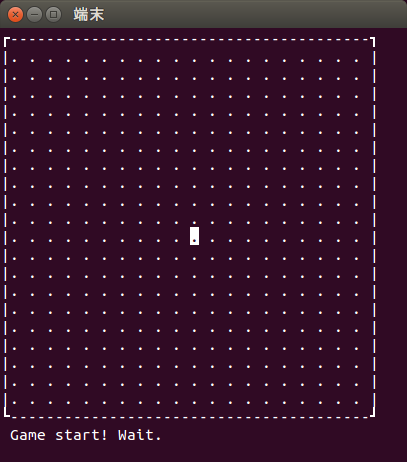
\includegraphics[scale=0.5]{img/game-start1.png}
    \caption{Caption}
    \label{fig:game-start1.png}
  \end{minipage}
  \begin{minipage}{0.5\hsize}
    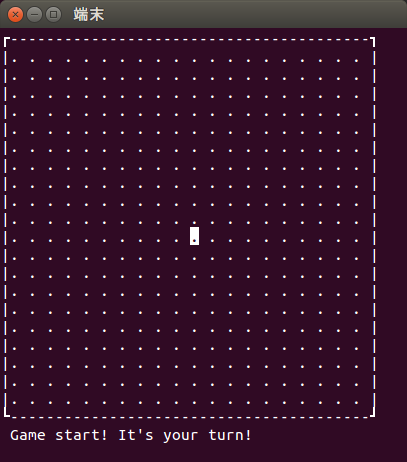
\includegraphics[scale=0.5]{img/game-start2.png}
    \caption{Caption}
    \label{fig:game-start2.png}
  \end{minipage}
\end{figure}


\begin{figure}[H]
  \begin{minipage}{0.5\hsize}
    \centering
    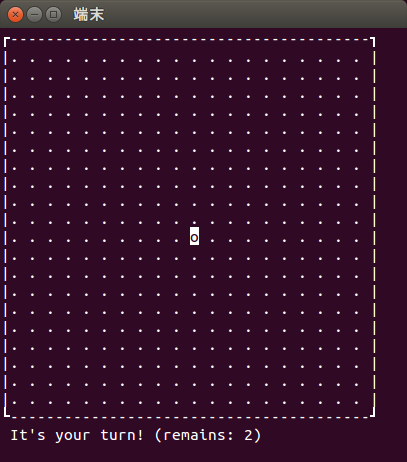
\includegraphics[scale=0.5]{img/put1-1.png}
    \caption{Caption}
    \label{fig:put1-1.png}
  \end{minipage}
  \begin{minipage}{0.5\hsize}
    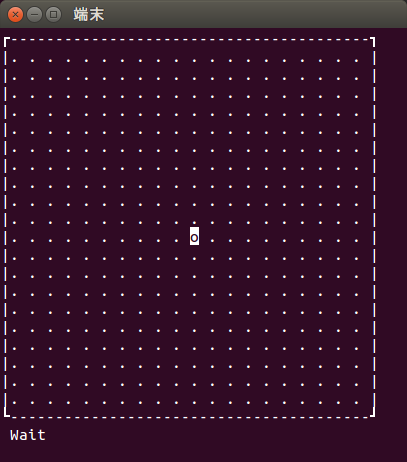
\includegraphics[scale=0.5]{img/put1-2.png}
    \caption{Caption}
    \label{fig:put1-2.png}
  \end{minipage}
\end{figure}

\begin{figure}[H]
  \begin{minipage}{0.5\hsize}
    \centering
    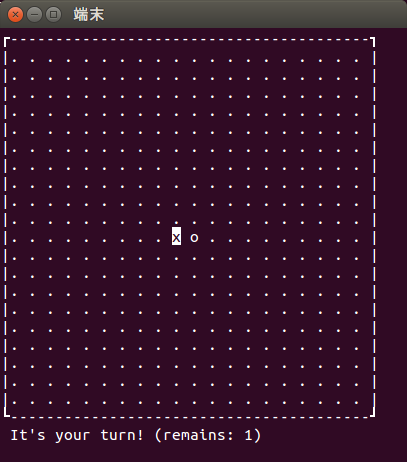
\includegraphics[scale=0.5]{img/put2-1.png}
    \caption{Caption}
    \label{fig:put2-1.png}
  \end{minipage}
  \begin{minipage}{0.5\hsize}
    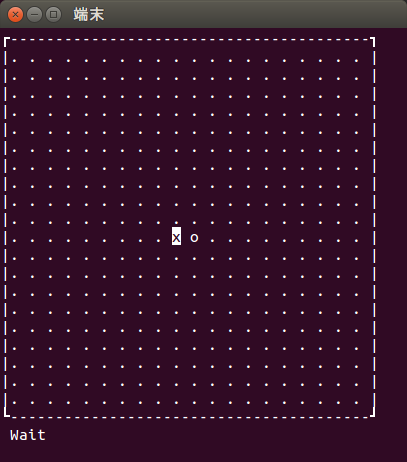
\includegraphics[scale=0.5]{img/put2-2.png}
    \caption{Caption}
    \label{fig:put2-2.png}
  \end{minipage}
\end{figure}

\begin{figure}[H]
  \begin{minipage}{0.5\hsize}
    \centering
    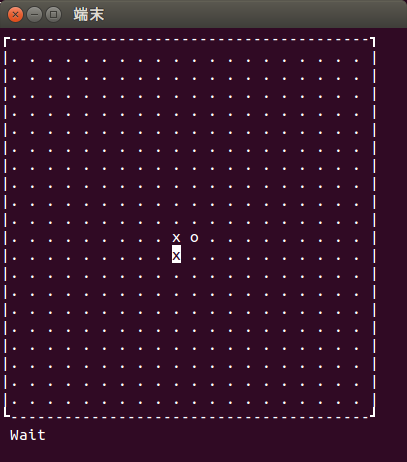
\includegraphics[scale=0.5]{img/put3-1.png}
    \caption{Caption}
    \label{fig:put3-1.png}
  \end{minipage}
  \begin{minipage}{0.5\hsize}
    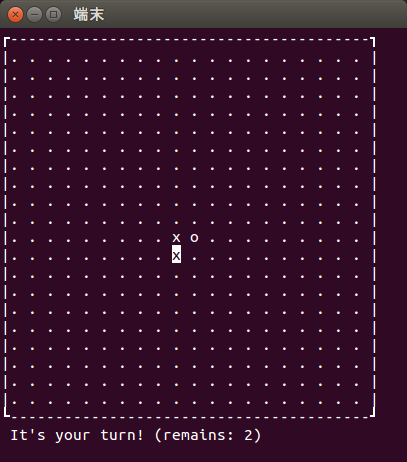
\includegraphics[scale=0.5]{img/put3-2.png}
    \caption{Caption}
    \label{fig:put3-2.png}
  \end{minipage}
\end{figure}

\begin{figure}[H]
  \begin{minipage}{0.5\hsize}
    \centering
    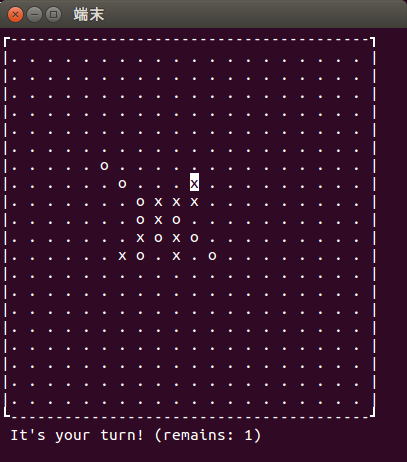
\includegraphics[scale=0.5]{img/fin-prev1-1.png}
    \caption{Caption}
    \label{fig:fin-prev1-1.png}
  \end{minipage}
  \begin{minipage}{0.5\hsize}
    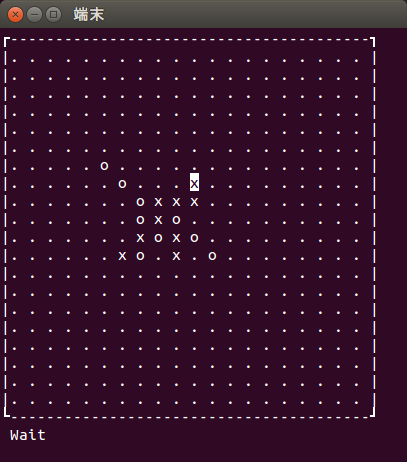
\includegraphics[scale=0.5]{img/fin-prev1-2.png}
    \caption{Caption}
    \label{fig:fin-prev1-2.png}
  \end{minipage}
\end{figure}

\begin{figure}[H]
  \begin{minipage}{0.5\hsize}
    \centering
    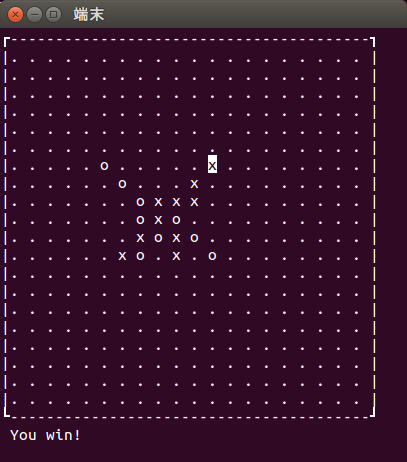
\includegraphics[scale=0.5]{img/fin-1.png}
    \caption{Caption}
    \label{fig:fin-1.png}
  \end{minipage}
  \begin{minipage}{0.5\hsize}
    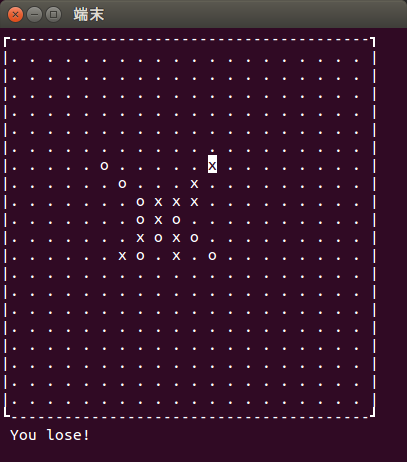
\includegraphics[scale=0.5]{img/fin-2.png}
    \caption{Caption}
    \label{fig:fin-2.png}
  \end{minipage}
\end{figure}


% ==============================================================================
\section{考察}


\end{document}
